\documentclass{article}
\usepackage{tikz}
\usetikzlibrary{arrows.meta, bending, decorations.markings, calc}
\usepackage{amsmath}

\begin{document}

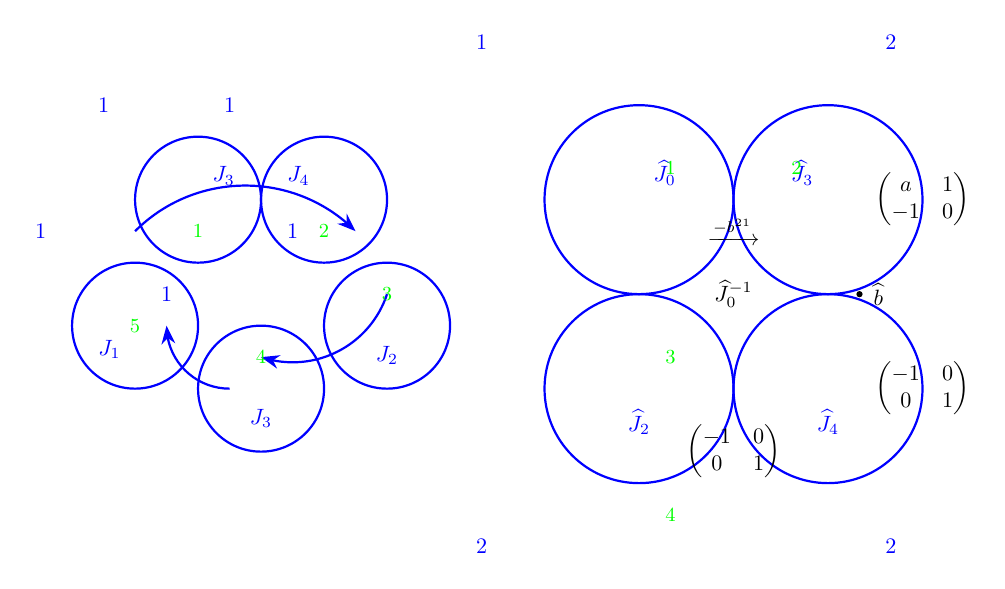
\begin{tikzpicture}[
    scale=0.8, 
    every node/.style={scale=0.8},
    arc_light/.style={-Stealth, densely dotted},
    arc_heavy/.style={-Stealth, thick, blue},
    decoration={markings, mark=at position 0.5 with {\arrow{Stealth}}}
    ]
    
    % Left diagram
    \draw[arc_heavy] (0,0) coordinate (J0) circle (1cm) node[above right=1mm] {$J_3$} node[xshift=-1.5cm, yshift=1.5cm] {$1$};
    \draw[arc_heavy] (2,0) coordinate (J1) circle (1cm) node[above left=1mm] {$J_4$} node[xshift=-1.5cm, yshift=1.5cm] {$1$};
    \draw[arc_heavy] (3,-2) coordinate (J2) circle (1cm) node[below=2mm] {$J_2$} node[xshift=-1.5cm, yshift=1.5cm] {$1$};
    \draw[arc_heavy] (1,-3) coordinate (J3) circle (1cm) node[below=2mm] {$J_3$} node[xshift=-1.5cm, yshift=1.5cm] {$1$};
    \draw[arc_heavy] (-1,-2) coordinate (J4) circle (1cm) node[below left=1mm] {$J_1$} node[xshift=-1.5cm, yshift=1.5cm] {$1$};
    \draw[arc_heavy] (-1, -0.5) to[bend left=45] (2.5, -0.5);
    \draw[arc_heavy] (3, -1.5) to[bend left=45] (1, -2.5);
    \draw[arc_heavy] (0.5, -3) to[bend left=45] (-0.5, -2);
    
    % Right diagram
    \begin{scope}[xshift=7cm]
        \draw[arc_heavy] (0,0) coordinate (J0t) circle (1.5cm) node[above right=1mm] {$\widehat{J}_0$} node[xshift=-2.5cm, yshift=2.5cm] {$1$};
        \draw[arc_heavy] (3,0) coordinate (J3t) circle (1.5cm) node[above left=1mm] {$\widehat{J}_3$} node[xshift=1cm, yshift=2.5cm] {$2$};
        \draw[arc_heavy] (3,-3) coordinate (J4t) circle (1.5cm) node[below=2mm] {$\widehat{J}_4$} node[xshift=1cm, yshift=-2.5cm] {$2$};
        \draw[arc_heavy] (0,-3) coordinate (J2t) circle (1.5cm) node[below=2mm] {$\widehat{J}_2$} node[xshift=-2.5cm, yshift=-2.5cm] {$2$};
        
        \node at (4.5,0) {$\begin{pmatrix}a & 1 \\ -1 & 0\end{pmatrix}$};
        \node at (4.5,-3) {$\begin{pmatrix}-1 & 0 \\ 0 & 1\end{pmatrix}$};
        \node at (1.5,-1.5) {$\widehat{J}_0^{-1}$};
        \node at (1.5,-4) {$\begin{pmatrix}-1 & 0 \\ 0 & 1\end{pmatrix}$};
        \node at (1.5, -0.5) {$\xrightarrow{-b^{21}}$};
        \node[fill, circle, inner sep=1pt] at (3.5, -1.5) {};
        \node[anchor=west] at (3.6, -1.5) {$\widehat{b}$};
    \end{scope}
    
    % Green numbering
    \begin{scope}[green]
        \foreach \x/\y/\num in {0/-0.5/1, 2/-0.5/2, 3/-1.5/3, 1/-2.5/4, -1/-2/5} {
            \node[font=\small] at (\x, \y) {\num};
        }
        \foreach \x/\y/\num in {7.5/0.5/1, 9.5/0.5/2, 7.5/-2.5/3, 7.5/-5/4} {
            \node[font=\small] at (\x, \y) {\num};
        }
    \end{scope}
\end{tikzpicture}

\end{document}